\chapter[Numerus- und Kasusmarkierung]{Numerus- und Kasusmarkierung und systematische Variation im syntaktischen Kontext}
\label{chap:9}\largerpage
Im Fokus der \chapref{chap:7} und \ref{chap:8} stand das isolierte Substantiv ohne Bezug zum syntaktischen Kontext. Der Phänomenbereich wird in diesem Kapitel auf die syntaktische Einheit der Nominalphrase bestehend aus Definitartikel und Substantiv erweitert. \sectref{sec:9.1} ist dabei stärker sprachsystematisch ausgerichtet, indem zunächst die dialektalen Artikelsysteme eingeführt und die Kodierung der Numerus- und Kasusinformation in der Nominalphrase dargestellt werden. Zu den Leitfragen dieses Kapitels gehören: In welchem Umfang und in welchen Konstellationen gibt es Synkretismen in den dialektalen Artikelsystemen? Wo wird die Numerus- und die Kasusinformation in der Nominalphrase markiert? Inwiefern werden Synkretismen in der Substantivflexion durch numerus- und kasuseindeutige Artikel kompensiert? Inwiefern werden wiederum Syn\-kretismen bei Artikelformen durch formale Kodierung am Substantiv kompensiert?

Synkretismen und flexivische Distinktionen bilden auch den Kern von \sectref{sec:9.2}, allerdings wird hier stärker der Sprachgebrauch unter Berücksichtigung des se"-man"-tisch-""prag"-ma"-tischen Kontexts fokussiert. Ganz im Sinne eines Dialektlabors kann gezeigt werden, dass sich in den oobd. Dialekten verschiedene Strategien herausgebildet haben, um mit gleichen Voraussetzungen, nämlich Synkretismen in der Substantivflexion, umzugehen. In einem Teil der bair. Dialekte ist Variabilität in der Kodierung flexivischer Information in Form von optionalen (sogenannten fakultativen) Markierungen sogar als morphologisches Prinzip grammatikalisiert.


Da die Untersuchung auch hier auf die Abfrage-Items und die Transkriptionen des BSA-Datenmaterials angewiesen ist, können in den folgenden Kapiteln nur einzelne Fallbeispiele diskutiert werden. Grenzen sind da gesetzt, wo die Berücksichtigung von verschiedenen syntaktischen Kontexten und der Informationsstruktur notwendig wäre, um Flexion an der Schnittstelle zur Syntax und zum semantisch-pragmatischen Kontext systematisch darzustellen. Trotz dieser Einschränkungen können mit den vorhandenen Daten bisherige Darstellungen ergänzt und gleichzeitig um einige interessante Forschungsperspektiven erweitert werden.

\section{Dialektale Artikelsysteme und flexivische Kodierung in der Nominalphrase}
\label{sec:9.1}
Für die Artikel- und Pronominalflexion können im Raum verschiedene Grade und Konstellationen von Synkretismen im Paradigma beschrieben werden (ausführlicher hierzu \citealt{Shrier1965}). Raumbildend sind aber nicht nur Synkretismuskonstellationen, sondern auch Aspekte funktionaler Variation in den dialektalen Artikelsystemen (vgl. den Überblick in \citealt[169]{Glaser2017}). Zu den Phänomenen, die in den untersuchten Dialekten zu finden sind, gehören die Verdopplung des Artikels in erweiterten Nominalphrasen (\textit{des ganz des kloane} ‚das ganz kleine (Schaf)‘, \textit{ein so ein schöner Tag}),\footnote{Vgl. \citealt[Karten 1B, 2B, 3B]{SNiB1} sowie \citet{StrobelWeiß2017}.} präpositionale Dativmarkierungen im Bair. (\textit{gibs α da Kathi} ‚gib es der Kathi‘),\footnote{Vgl. \citealt[Karte 5N]{SNiB1}.} die doppelte Reihe des Definitartikels („betonter“ Definitartikel \textit{di Frau} vs. „unbetonter“ Definitartikel \textit{de} oder \textit{d’Frau}) sowie der indefinite Pluralartikel im Mittelbair. (\textit{da hund hod α/oi flöh} ‚Der Hund hat Flöhe‘, \textit{mägsd a kersch} ‚Möchtest du Kirschen?‘).\footnote{Die Beispiele stammen aus \citet{Glaser1996} sowie aus \citealt[Karte 2C, vgl. Karten 3C und 5C]{SNiB1}.} Die Nominalphrase \textit{a kersch} ‚Kirschen‘ ist hier bemerkenswert, da sie hinsichtlich der Numerusinformation ambig ist: Die Indefinitartikel des Singular und des Plural sind im Femininum formal identisch, und am Substantiv selbst erfolgt keine formale Pluralmarkierung (vgl. \citealt[160]{Glaser1996}). Eine weitere formale und funktionale Besonderheit des Mittelbair. besteht darin, dass die Differenzierung von Definit- und Indefinitartikel des Maskulinums im Akk.Sg. aufgehoben ist und so ambige Formen hinsichtlich der Definitheit entstehen: \textit{I sig an fuks} ‚Ich sehe einen/den Fuchs‘ (\citealt[150]{Glaser1996}, vgl. \citealt[323]{Eroms1989}). Damit scheinen Formenambiguitäten ein konstitutiver Faktor der nominalen Morphosyntax in den untersuchten Dialekten zu sein, wobei im Einzelnen und durch geeignetes Datenmaterial noch zu klären ist, was etwa die Gebrauchs- und Geltungsbedinungen des indefiniten Pluralartikels sind und wie referentielle Ambiguitäten des Typs \textit{I sig an fuks} im Gesprächskontext disambiguiert werden (vgl. \citealt[160]{Glaser1996}).

\subsection{Synkretismuskonstellationen bei betontem und unbetontem Definitartikel}
\label{sec:9.1.1}
Im Bereich der Flexion des Definitartikels sind zwei unterschiedliche Synkretismuskonstellationen im Paradigma anzusetzen, die in \figref{fig:16} schematisiert sind. Im Maskulinum werden im Singular Nominativ und oblique Kasus differenziert (N/AD), bei Feminina, Neutra und im Plural werden eine synkretische Nominativ- und Akkusativform und eine distinkte Dativform unterschieden (NA/D).


\begin{figure}%9.1
\small
\begin{tikzpicture}
		\matrix [matrix of nodes,
		nodes in empty cells,
		column sep=3mm,
		align=center,
		nodes={text width=2cm, minimum height=1em, font=\strut},
		column 1/.style={nodes={text width=1cm}}
		]
		(matrix)
		{         & & {Singular} & & {Plural} \\
				  & Maskulinum & Neutrum & Feminimum & \\
			Nom.  & & & & \\
			Akk.  & & & & \\
			Dat.  & & & & \\
		};
		\draw (matrix-2-2.north west) -- (matrix-2-4.north east);
		\fill [fill=gray!20]
		(matrix-3-2.north west) rectangle (matrix-3-2.south east);
		\fill [fill=gray]
		(matrix-4-2.north west) rectangle (matrix-5-2.south east);
		\fill [fill=gray!20]
		(matrix-3-3.north west) rectangle (matrix-3-3.south east);
		\fill [fill=gray]
		(matrix-5-3.north west) rectangle (matrix-5-3.south east);
		\fill [fill=gray!20]
		(matrix-4-3.north west) rectangle (matrix-4-3.south east);
		\fill [fill=gray]
		(matrix-5-4.north west) rectangle (matrix-5-4.south east);
		\fill [fill=gray]
		(matrix-5-5.north west) rectangle (matrix-5-5.south east);
		\fill [fill=gray!20]
		(matrix-3-5.north west) rectangle (matrix-4-5.south east);
		\fill [fill=gray!20]
		(matrix-3-4.north west) rectangle (matrix-4-4.south east);
	\end{tikzpicture}
\caption{\label{fig:16}Synkretismuskonstellationen in den Definitartikelparadigmen}
\end{figure}

Im nordbair. Artikelsystem ist nach \citet[428]{Rowley1990b} eine dritte Synkretismuskonstellation (NAD) zu finden (vgl. \tabref{tab:40}). Neutra im Plural haben hier eine spezifische, kasussynkretische Form des Definitartikels: neutr. \textit{deiɐ ghinɐ} ‚die Kinder‘ vs. mask. \textit{die boum} ‚die Buben‘ (vgl. \teuthoo{de<E}{dêə} \teuthoo{mo<i.«d»lAn}{môiͅ(d)lαn} ‚den Mädchen‘ im nordbair. Groschlattengrün). Ein synkretischer Pluralartikel findet sich vereinzelt auch im Ofr. und (für alle Genera) im Nordbair. (vgl. \citealt[347]{Rowley2004}, \citealt[436]{SMF7}).\footnote{Z.\,B. mit betontem Artikel \teuthoo{îi“4}{{\aufstrih}ị̄} \teuthoo{mu<os}{mûos} \teuthoo{di}{di} \teuthoo{khu"?E.}{khǖəͅ} \teuthoo{vo?.dEr}{vöͅdər} ‚ich muss die Kühe füttern‘ und mit unbetontem Artikel \teuthoo{gab}{ɡab} \teuthoo{A4ma9.2}{α̣ma\klammeruntenpost{}̄ͅ} \teuthoo{dE}{də} \teuthoo{khu"?E.}{khǖəͅ} \teuthoo{wa.s}{waͅs} \teuthoo{dsu}{dsu} \teuthoo{v5ra4sE}{v̩rạsə} ‚gib einmal den Kühen was zum Fressen‘ (ofr. Erlabrunn) oder im nordbair.-mittelbair. Grafenkirchen: \teuthoo{de4}{dẹ} \teuthoo{k\_e.<i}{kʰêͅi} ‚die Kühe (kaufe ich nicht)‘ und \teuthoo{miE}{miə} \teuthoo{gemS}{ɡemʃ} \teuthoo{de4}{dẹ} \teuthoo{k\_e.<i}{kʰêͅi} ‚wir geben es den Kühen‘.}


\begin{table}[p]
\begin{tabular}{lllllll}
\lsptoprule
& \multicolumn{3}{c}{{Sg.}} & \\
 & {Mask.} & {Neutr.} & {Fem.} & \multicolumn{2}{c}{{Pl.}} & \multicolumn{1}{l}{{Neutr.}}\\\cmidrule(lr){2-4}\cmidrule(lr){5-6}\cmidrule(lr){7-7}
{Nom.} & \cellcolor{lsLightGray}\textit{dα} / \textit{deα} & \cellcolor{lsLightGray}\textit{(ə)s} / \textit{des} & \cellcolor{lsLightGray}\textit{d‘} / \textit{di} & \cellcolor{lsLightGray}\textit{d‘} / \textit{de}\footnote{Im nordbair. Groschlattengrün, wo sich keine klitisierten Artikelformen finden, lautet der unbetonte Pluralartikel \textit{di}, der betonte \textit{dei}.} & \cellcolor{lsLightGray}\textit{də} / \textit{di} & \textit{deiɐ}\\
{Akk.} & \cellcolor{lsLightGray}\textit{αn} / \textit{dαn} & \cellcolor{lsLightGray} & \cellcolor{lsLightGray} & \cellcolor{lsLightGray} & \cellcolor{lsLightGray} & \\
{Dat.} & \cellcolor{lsLightGray} & \textit{n} & \cellcolor{lsLightGray}\textit{dα} & \cellcolor{lsLightGray}\textit{(α)n} & \cellcolor{lsLightGray} & \\
\lspbottomrule
\end{tabular}
\caption{Flexionsparadigma des Definitartikels (unbetont\slash betont) im Nordbair. (vgl. \citealt[427]{Rowley1990b}). Die Paradigmen stellen eine Abstraktion der heteromorphischen Varianten dar, d.\,h. im Einzeldialekt können die Artikelformen anders realisiert werden. Grau hinterlegt sind in dieser und in den folgenden Tabellen die Paradigmenpositionen, die durch die eigenen BSA-Daten gefüllt werden konnten; die weiß hinterlegten Angaben stammen von \citet[403]{Rowley1990a}, \citet[427]{Rowley1990b} zum Nordbair. sowie \citet[316]{Eroms1989} und \citet[237]{Scheutz1988} zum Mittelbair.\label{tab:40}}
\end{table}

\begin{table}[p]
\begin{tabular}{llllll}
\lsptoprule
& {Mask.} & {Neutr.} & {Fem.} & \multicolumn{2}{c}{{Pl.}}\\\cmidrule(lr){2-4}\cmidrule(lr){5-6}
{Nom.} & \cellcolor{lsLightGray}\textit{dα} / \textit{deα} & \cellcolor{lsLightGray}\textit{əs} / \textit{des} & \cellcolor{lsLightGray}\textit{də} / \textit{di} & \cellcolor{lsLightGray}\textit{di} & \cellcolor{lsLightGray}\textit{də} / \textit{di}\\
{Akk.} & \cellcolor{lsLightGray}\textit{(α)n} / \textit{dαn} & \cellcolor{lsLightGray} & \cellcolor{lsLightGray} & \cellcolor{lsLightGray} & \cellcolor{lsLightGray}\\
{Dat.} & \cellcolor{lsLightGray} & \textit{ən} / \textit{den} & \cellcolor{lsLightGray}\textit{dα} / \textit{deα} & \textit{ən} / \textit{den} & \cellcolor{lsLightGray}\\
\lspbottomrule
\end{tabular}
\caption{Flexionsparadigma des Definitartikels (unbetont\slash betont) im Ofr. (vgl. \citealt[403]{Rowley1990a} sowie \citealt[189]{SUF3} speziell zum Unterofr.). Beim Nom.\slash Akk. der Feminina wurde in den ausgewerteten BSA-Daten jeweils nur die Form \textit{di} realisiert; hier kann allerdings auch eine unbetonte Form \textit{də} angenommen werden, die in den ofr. Ortsdialekten mit vollständigem Kasussynkretismus im Fem. im Satzkontext produziert wurde.\label{tab:41}}
\end{table}

\begin{table}[p]
\begin{tabular}{lllll}
\lsptoprule
& {Mask.} & {Neutr.} & {Fem.} & {Pl.}\\\midrule
{Nom.} & \cellcolor{lsLightGray}\textit{dα} / \textit{deα} & \cellcolor{lsLightGray}\textit{(α)s} / \textit{des} & \cellcolor{lsLightGray}\textit{d‘} / \textit{de} & \cellcolor{lsLightGray}\textit{d‘} / \textit{de}\\
{Akk.} & \cellcolor{lsLightGray}\textit{αn} / \textit{dαn} & \cellcolor{lsLightGray} & \cellcolor{lsLightGray} & \cellcolor{lsLightGray}\\
{Dat.} & \cellcolor{lsLightGray} & \textit{an} / \textit{den} & \cellcolor{lsLightGray}\textit{dα / dera} & \textit{de} / \textit{dene}\\
\lspbottomrule
\end{tabular}
\caption{Flexionsparadigma des Definitartikels (unbetont\slash betont) im Mittelbair. (vgl. \citealt[316]{Eroms1989}, \citealt[237]{Scheutz1988})}
\label{tab:42}
\end{table}

Auch wenn in den eigenen Daten hierfür keine Belege gefunden wurden, so wird in dialektologisch-grammatischen Darstellungen außerdem eine Tendenz zum Kasussynkretismus bei den Feminina für Teile des Ofr. beschrieben. \citet[Karte 6]{Shrier1965} setzt für einen Ortspunkt im Unterofr. den völligen Zusammenfall der Kasusdifferenzierung beim fem. Definit- und Indefinitartikel an, mit \textit{də} als synkretischem fem. Definitartikel. \citet[§6d]{Schübel1955} sieht den „Bestand und Bereich“ des Dativs „stark bedroht“; im ofr. Stadtsteinach findet sich die Variante \teuthoo{ic}{iX} \teuthoo{ho2us}{hōus}  \teuthoo{di}{di} \teuthoo{fra2}{frā} \teuthoo{ge2m}{ɡēm} ‚Ich hab’s der Frau gegeben‘ neben \teuthoo{ic}{iX} \teuthoo{ho2us}{hōus} \teuthoo{da?}{dä} \teuthoo{fra2}{frā} \teuthoo{ge2m}{ɡēm}. Auch \citet[92]{Rowley1997} beschreibt für dieses oberofr. Gebiet eine Entwicklung hin zu völligem Kasussynkretismus bei den Feminina. Die Varianten \teuthoo{nai}{nai} \teuthoo{di}{di} \teuthoo{windEriN}{windəriŋ} vs. \teuthoo{nai}{nai} \teuthoo{dE}{də} \teuthoo{windEriN}{windəriŋ} ‚(die Karpfen kommen) hinein die Winterunterbringung‘,\footnote{Zur Verwendung und Arealität von Lage- und Richtungsadverbien als Präpositionen im Ofr. vgl. den Forschungsüberblick und die Ergebnisse im SMF (\citealt[434--438]{SMF7}, vgl. auch \citealt{WA}-Karten 28, 56, 467 „in“).}  die sich „in kurzer Abfolge“ finden, sind \citet[92]{Rowley1997} zufolge auf die durch den Satzakzent bedingte Verwendung des betonten und des unbetonten (d.\,h. nicht akzentuierbaren) Artikels zurückzuführen. Demnach wären hier zwei unterschiedliche, aber jeweils synkretische Paradigmen anzusetzen: Nom./Akk./Dat. \textit{di} als betonter und Nom.\slash Akk./Dat. \textit{də} als unbetonter Definitartikel.

Diese beiden Reihen des Artikels, d.\,h. Vollformen vs. reduzierte Formen, müssen für alle untersuchten Dialekte angesetzt werden (vgl. 	\tabref{tab:40} bis \tabref{tab:42}). Allerdings ist die Distribution der beiden Artikelformen nicht nur durch Akzent und Position bedingt, sondern auch durch unterschiedliche Funktionalitäten im semantisch-pragmatischen Kontext (siehe hierzu
\citealt{Eroms1989}, \citealt{Scheutz1988}, \citealt{WeißDirani2019}). Im BSA-Fragebuch wurden die beiden Reihen des Definitartikels zwar berücksichtigt, etwa durch die Fragen „Die Häuser (betont!) gefallen uns nicht“ oder „Die Kühe (unbetont!) kauf‘ ich nicht“, allerdings ist das Datenmaterial außerhalb dieser elizitierten Syntagmen zu heterogen und zu wenig eindeutig, um auf die Distribution von Voll- und reduzierten Formen zu schließen.\footnote{Bedingt durch die Datenlage lassen sich daher nur einzelne Beobachtungen aufführen, da Definitartikel für einzelne Paradigmenposition gar nicht oder nur in Form eines Abfrage-Items vorliegen (vgl. die Problematisierung in \sectref{sec:7.2}). Erschwert wird die Auswertung dadurch, dass eine Klassifikation und Differenzierung nach Kasus anhand der Transkriptionen (und der wenigen Abfrage-Items) nicht immer eindeutig ist, insbesondere wenn der Artikel in der reduzierten Form vorkommt (siehe auch \citealt[189]{SUF3}). Bedingt durch die Art der Datenerhebung kommen mögliche Intervieweffekte hinzu (zumeist isolierte Antwort-Items und die Elizitierung der relevanten NPs in der Vorfeld-Position), die die Realisierung der Artikelform (Vollform oder reduzierte Form) beeinflussen.} Des Weiteren haben \citet[330]{WeißDirani2019} in ihrer Studie zum hess. Definitartikelsystem jüngst gezeigt, dass für die Funktionalität der beiden Definitartikelformen insbesondere mit Blick auf Faktoren der Informationsstruktur „a more fine-grained differentiation“ angesetzt werden muss, als bisher angenommen. Um die Distribution der Artikelformen in den Dialekten abbilden zu können, braucht es dementsprechend Datenmaterial, das die verschiedenen morphosyntaktischen und informationsstrukturellen Faktoren systematisch berücksichtigt (vgl. \citealt[239--240]{Scheutz1988}).\footnote{Siehe hierzu als Beispiel die Erhebungen des SNiB, wo die Verwendung von reduzierter vs. Vollform bei einfachen Wiederaufnahmesituationen eliziert und Spontanantworten vs. akzeptierte Antworten systematisch differenziert wurden (\citealt[130]{SNiB1}).}

In den bair. Dialekten wird die unbetonte Artikelform \textit{die} im Nominativ/Akkusativ der Feminina und des Plurals als Proklise realisiert, z.\,B. (mit Assimilation des Artikels) \teuthoo{b-mu<94AtE}{b{}͐mû\klammeruntenpost{}̣αtə} -- \teuthoo{b-mu42AtEn}{b{}͐mụ̄αtən} ‚Mutter‘ im mittelbair. Grafenau, \teuthoo{svenStA}{svenʃtα} -- \teuthoo{b,venStA}{b͓venʃtα} ‚Fenster‘ im nordbair. Nabburg (vgl. \citealt[112--114 und Karte 18]{Rowley1997}, \citealt[§449]{Schmeller1821}). Variation besteht in den Dialekten dahingehend, ob der Definitartikel auch positionsbedingt vor einem Adjektivattribut reduziert werden kann: \textit{s’laar(e)} vs. \textit{des laar(e) Glas} ‚das leere Glas‘, \textit{d’schene} vs. \textit{de schene} ‚die schöne (Huberbäuerin)‘. Dieser Aspekt wurde im Band 1 des \textit{Sprachatlas von Niederbayern} systematisch erhoben und ausgewertet, und es zeigt sich, dass bei Neutra und noch stärker bei den Feminina die Vollform gegenüber der klitisierten Form präferiert wird (\textit{de schene} vs. \textit{d’schene}), während bei den Maskulina die reduzierte Form \textit{dα oi(te)} gegenüber der Vollform \textit{deα oi(te)} ‚der alte (Bauer)‘ präferiert wird (\citealt[108--130]{SNiB1}, vgl. \citealt[317]{Eroms1989}). Auch in den untersuchten Dialekten erscheint vor Adjektivattribut eher die Vollform des Artikels als die reduzierte Form (tatsächlich findet sich kein Beleg für Artikelproklise vor Adjektiv\-attribut).

Mit Blick auf die formale Realisierung der Definitartikel und deren Distribution sind daneben auch Sandhi-Effekte zu beobachten. In Flexionssystemen, die keine Distinktion zwischen Dativ und Akkusativ im Singular des Maskulinums oder Neutrums haben, ist zum Teil eine progressive Assimilation des Definitartikels \textit{αn} > \textit{αm} zu finden (Typ \textit{Ghead des an Hans oda am Franz} ‚Gehört das dem Hans oder dem Franz‘, \citealt[09]{Zehetner1985}): Akk.Sg. \teuthoo{Am}{αm} \teuthoo{b5a4<o<n}{b̩ậôn} ‚Bauer‘ vs. Akk.Sg. \teuthoo{An}{αn} \teuthoo{s\#po.2ds}{špōͅds} ‚Spatz‘ (mittelbair. Wolfersdorf), \teuthoo{Am}{αm} \teuthoo{be4<Ag}{bệαɡ} \teuthoo{a4ofi}{ạof‌i} ‚auf den Berg hinauf‘ (mittelbair. Wolfersdorf) vs. \teuthoo{An}{αn} \teuthoo{b\%eAg}{b͈eαɡ} \teuthoo{a4u:fe}{ạu{\doubleogonek}fe} ‚auf den Berg hinauf‘ (mittelbair. Inning am Holz, vgl. \citealt[§3d]{Schübel1955}). Daneben bietet \citet[§59]{Freudenberg1959} einen Beleg dafür, dass in Flexionssystemen, in denen Akkusativ und Dativ unterschieden werden, diese Differenzierung durch Assimilation aufgehoben werden kann: mittelbair. \teuthoo{i}{i} \teuthoo{ha2sn@}{hāsn̥} \teuthoo{ge2wA}{ɡēwα} ‚ich habe es ihm gegeben‘.

\subsection{Kasusmarkierung in der Nominalphrase}\label{sec:9.1.2}
Im UG besteht Variation dahingehend, welche Kasus durch Präpositionen regiert werden. Bei den Richtungsadverbien in präpositionaler Funktion im Ofr. sind variante Kasusrektionen auch raumbildend, z.\,B \textit{hinauf der Eiche} mit Dativrektion vs. \textit{hinauf die Eiche} mit Akkusativrektion (\citealt[435--436 und Karten 121--125]{SMF7}). Grundsätzlich zu unterscheiden sind Dialektsysteme, in denen Präpositionen immer den Dativ regieren, wie es \citet[93]{Rowley1997} für die konservativen ofr. Dialekte beschreibt, und jene, in denen Akkusativ und Dativ regierende Präpositionen unterschieden werden, beispielsweise \teuthoo{a4v5}{ạv̩} \teuthoo{d5o<).AxA}{d̩ô\klammeruntenpost{}ͅαxα} ‚auf der Eiche‘ vs. \teuthoo{untA4}{untα̣} \teuthoo{dE}{də} \teuthoo{o.AxE}{oͅαxə} ‚unter der Eiche‘ im mittelbair. Grafenau. Auch im südlichen Unterofr. und dem westlichen Streifen des Ofr. werden Präpositionen mit Akkusativ- und Dativrektion unterschieden, doch erscheint in einem relativ geschlossenen Gebiet nach dativregierenden Präpositionen numerusunabhängig der Definitartikel \textit{der}: \teuthoo{An}{αn} \teuthoo{dEr}{dər} \teuthoo{hend5\_}{hend̩ʰ} ‚an den Händen‘ (ofr. Gebsattel), \teuthoo{na2}{nā} \teuthoo{BE}{{\btilde}ə} \teuthoo{dEr}{dər} \teuthoo{a.ldi}{aͅldi} \teuthoo{ho<I?sEr}{hôı̈sər} ‚nahe bei den alten Häusern‘ (ofr. Ochsenfurt), \teuthoo{mi.dEr}{miͅdər} \teuthoo{bu2Em}{būəm} ‚mit den Buben‘ (ofr. Hüttenheim, vgl. \citealt[Karte 56]{SUF3}).

Ein Beispiel für die Variabilität flexivischer Kodierung in der Nominalphrase bieten jene nordbair. und ofr. Dialekten, die eine distinkte Dativ-Plural-Form haben. Exemplarisch zeigt dies die Belegreihe \teuthoo{mitE}{mitə}
\teuthoo{g\_\i“En@}{ɡʰ̈īən̥} ‚mit der Kette‘ vs. \teuthoo{mi}{mi} \teuthoo{k\_i“ErAn}{kʰīərαn} ‚mit Ketten‘ aus dem nordbair. Windischeschenbach: Der Definitartikel entfällt, wenn eine flexivische Markierung der Kasus- und Numerusinformation am Substantiv zu Verfügung steht. In der Nominalphrase besteht also eine Tendenz zur Monoflexion, es findet eine „Arbeitsteilung der nominalflexivischen Kennzeichnung“ \citep[387]{Harnisch2019} statt: entweder am Substantiv oder am Artikel.

In Dativ regierten Präpositionalphrasen mit pluralischer Nominalphrase wird die flexivische Information in diesen Dialekten präferiert am Substantiv kodiert; der Artikel wird entweder reduziert (klitisiert) realisiert oder es erscheint kein Artikel: \teuthoo{avÑ}{av{\burgermn}} \teuthoo{ba42mana}{bạ̄mana} ‚auf den Bäumen‘ (ofr. Hallerstein), \teuthoo{in}{in} \teuthoo{a4rmAn}{ạrmαn} ‚in den Armen‘ (nordbair. Tirschenreuth), \teuthoo{a4m}{ạm} \teuthoo{ne4s5dnAn}{nẹs̩dnαn} \teuthoo{dra.n}{draͅn} ‚an den Ästen dran‘ (nordbair.-mittelbair. Blaibach). Diese Belege sind auch insofern bemerkenswert, als \citet[95]{Rowley1997} für in sein nordostbayerisches UG nach Präposition eher die Form ohne Dativ-Plural-Suffix anführt.\largerpage[2]

\begin{sloppypar}
Beispiele für morphosyntaktische Varianten nach Präposition bietet auch \citet[§13]{Schübel1955} für den ofr. Dialekt von Stadtsteinach: \textit{mid di bȳχe} -- \textit{midn bȳχenɐ} ‚mit den Büchern‘, \textit{họie šded negs auf di fäle} -- \textit{aufm fälenɐ} ‚heuer steht nichts auf den Feldern‘. Des Weiteren zeigt \citet[§13]{Schübel1955}, dass auch Kasuswechsel am Artikel in Kauf genommen wird, um Numerus eindeutig zu markieren.\footnote{Auch \citet[§12]{Weitzenböck1942} bietet Belege dafür, dass Numerusambiguitäten in der Präpositionalphrase durch eine andere Kasusmarkierung am Artikelwort aufgelöst werden: mittelbair. \teuthoo{fo}{fo} \teuthoo{ma+n}{mãn} \teuthoo{fe24dA+n}{fẹ̄dα̃n} ‚von meinem/meinen Vetter(n)‘ wird zu \teuthoo{fo}{fo} \teuthoo{ma+ne4}{mãnẹ} \teuthoo{fe24dA+n}{fẹ̄dα̃n} ‚von meinen Vettern‘ mit dem Possessivartikel im Akk.Pl., wenngleich dieser „nicht bodenständige [d.\,h. basisdialektale, GN] Ersatz aus der städtischen Sprache“ und anderen Dialekten stamme und „offenbar im Vordringen“ sei.} Im Syntagma \textit{en báuen kǫsdɒ šö dráun} ‚dem/den Bauern kannst du schon trauen‘ liegt durch den synkretischen Artikel \textit{en} (Akk./Dat.Sg.mask. und Dat.Pl.) Numerusambiguität vor, die entweder flexivisch am Substantiv oder durch den Pluralartikel des Nom./Akk. (\textit{di}) vereindeutigt wird: \textit{en báuenɒ} oder \textit{di báuen} \textit{kǫsdɒ šö dráun} ‚den Bauern kannst du schon trauen‘ (siehe auch \sectref{sec:7.2.2}). \citet[123--124]{Steininger1994} zufolge wäre im Flexionssystem des mittelbair. Oberneureutherwaid der „potenzierte Plural“ in der Form des Dat.Pl. bei der synkretischen Artikelform \textit{en} obligatorisch (\textit{bis’a én Buaman schreid} ‚bis er die Buben weckt‘), während er in einer NP mit distinktem Artikel (Dat.Sg. \textit{dän} -- Pl. \textit{dé}) „sogar ungrammatisch“ wäre: \textit{Dé Buam} (*\textit{dé Buaman}) \textit{gibd’a oiss} ‚Den Buben gibt er alles‘.
\end{sloppypar}

Während die formale Variabilität bei der Kodierung der flexivischen Information in diesen Fällen der Disambiguierung der Numerusinformation dient, hat sich im Bair. (neben anderen obd. Dialekten) eine weitere dialektspezifische Strategie zur Kodierung der Kasusinformation des Dativs herausgebildet: die präpositionale Dativmarkierung des Typs \textit{gibs α da Kathi} ‚gib es der Kathi‘. Im Mittelbair. ist bei den reduzierten Definitartikelformen des Plurals Kasusdistinktion vorhanden (Nom./Akk.Pl. \textit{d’leit} vs. Dat.Pl. \textit{de leit} ‚Leute‘), nicht aber bei den Vollformen: Nom./Akk./Dat.Pl. \textit{de leit} \citep[98--99]{Seiler2003}. \citet[150]{Seiler2003} analysiert die präpositionale Dativmarkierung als „eine Angelegenheit der Ausbuchstabierung des Dativs“, indem der Marker den Kasus der folgenden NP explizit markiert und vor dem Hintergrund einer Präferenz von Dativ in Kookkurrenz mit vorangehender Präposition heraus zu verstehen ist; der Dativmarker hat damit die „Funktion eines Expletivs, eines Platzhalters“ \citep[148]{Seiler2003}. Aus flexionsmorphologischer Perspektive ist hierbei \citegen[166]{Seiler2003} Befund zentral, dass der Dativmarker v.\,a. im Südbair. und teilweise im Mittelbair. häufiger im Plural als im Singular vorkommt, das heißt da, wo Synkretismen in der Nominalphrase vorliegen (\textit{di leit} vs. \textit{in di leit} ‚den Leuten‘). Hier hat die präpositionale Dativmarkierung eine disambiguierende Funktion.

Insgesamt erscheint der präpositionale Dativmarker im Bair. eher mit Definitartikel, so auch in einem Teil der untersuchten mittelbair. Dialekte: \teuthoo{A}{α} \teuthoo{dA}{dα} \teuthoo{mu<AtA}{mûαtα} \teuthoo{gðs5o.gd}{ɡ̩s̩oͅɡd} ‚der Mutter gesagt‘ und \teuthoo{A}{α} \teuthoo{d5e4n}{d̩ẹn} \teuthoo{o.idn}{oͅidn} \teuthoo{mo4"+}{mọ̃̄} ‚dem alten Mann (gegeben)‘ in Kirchensur (vgl. \citealt[106--110]{Seiler2003}). Seltener und unregelmäßiger verteilt ist die präpositionale Dativmarkierung nach De"-mons"-tra"-tiv-,"" Pos"-ses"-siv-"" oder In"-ter"-ro"-ga"-tiv"-ar"-ti"-kel, z.\,B. \teuthoo{A}{α} \teuthoo{de4<}{dệ} \teuthoo{we4<cAn}{wệXαn} \teuthoo{k\_i."4ndA}{kʰị̄ͅndα} ‚welchen Kindern (hast du es gegeben)‘ in Reischach. Das Auftreten des Dativmarkers ist dabei „mehr oder weniger optional“ \citep[152]{Seiler2003}, {{dativische}} Nominalphrasen kommen etwa im mittelbair. Niedertaufkirchen auch ohne präpositionalen Dativmarker vor: \teuthoo{A}{α} \teuthoo{dA}{dα} \teuthoo{mu.<AtAn}{mûͅαtαn} \teuthoo{ks5o.k,t,\_}{ks̩oͅk͓t͓ʰ} ‚der Mutter gesagt‘ vs. \teuthoo{de4n}{dẹn} \teuthoo{o4<e4dn@}{ộẹdn̥} \teuthoo{ma.>(+}{mẫͅ\klammerobenpost{}} ‚dem alten Mann (gegeben)‘. Grundsätzlich ist das Auftreten der präpositionalen Dativmarkierung an keine semantischen Distinktionen gekoppelt, sie kodiert keine semantischen Rollen. Nach \citet[187]{Seiler2003} stellen aber informationsstrukturelle Aspekte in den Dialekten mit optionaler präpositionaler Dativmarkierung einen Auftretensfaktor dar: „Je mehr eine dativische NP diskursfunktional markiert ist, desto eher wird sie präpositional markiert.“

Diese Zusammenschau an Phänomenen zeigt, dass sich in den dialektalen Flexionssystemen spezifische Strategien zur Vereindeutigung von Numerus- oder Kasusinformation finden, die erst im morphosyntaktischen Kontext greifen. Im Falle der präpositionalen Dativmarkierung sind diese sogar grammatikalisiert. Vor dem Hintergrund von Numerusprofilierung und Kasusnivellierung als zentralen Tendenzen nominalmorphologischen Wandels ist gleichzeitig bemerkenswert, dass in einzelnen Dialektsystemen Kasuswechsel des Artikels in Kauf genommen werden, um eine eindeutige Kodierung der Numerusinformation sicherzustellen. Insgesamt entsprechen die dialektalen Strategien im UG auch der Beobachtung \citegen[436]{Shrier1965}, dass (morpho-)syntaktische Ambiguitäten als Folge von Synkretismen durch weiteren Kontext und kommunikative Strategien disambiguiert werden.

\section{Systematische Variation der Pluralmarkierung im syntaktischen Kontext}
\label{sec:9.2}
In den Kapiteln zur Formenbildung und zum dialektalen Deklinationsklassensystem wurde punktuell immer wieder vermerkt, dass die eine oder andere distinkte Markierung in dialektologisch-grammatischen Darstellungen als fakultativ (d.\,h. als optional) klassifiziert wurde:

\begin{itemize}
\sloppy
\item Im mittelbair. Dialekt von Oberneureutherwaid erscheinen keine Lenis-Fortis-Kontraste als Mittel der Numerusdifferenzierung, wenn der Plural bereits durch ein Zahlwort ausgedrückt wird: \textit{d̥iːʒ} -- \textit{d̥iʃ} ‚Tisch‘, aber \textit{t̥sβæ d̥i:ʒ} ‚zwei Tische‘ (\citealt[124]{Steininger1994}, siehe \sectref{sec:7.1.2.3.1}). Nach Zahlwort besteht nach \citet[105]{Rowley1997} grundsätzlich „die morphosyntaktische Option“, die unflektierte Form des Nom.Sg. zu verwenden, und zwar unabhängig von einer Semantik des Lexems als Maß- und Mengenangabe und vom jeweiligen Pluralmarkierungsverfahren (vgl. \sectref{sec:8.3.2}).
\item Im südlichen Nordbair. ist die additive Markierung durch Nasalsuffix von Maskulina mit Tiefschwa- und \textit{el}{}-Reduktionssilbe fakultativ (daneben auch bei Diminutiva auf -\textit{el}), wenn „der syntaktische Rahmen keine weiteren Hinweise auf die Pluralität liefert“ \citep[158]{Rowley1997} und der Stammvokal im Plural keinen Umlaut aufweist: Pl. \teuthoo{s\#lisln}{šlisln} vs. \teuthoo{tswaI2\textsuperscript{n}}{tswaı̄\textsuperscript{n}} \teuthoo{s\#lisl}{šlisl} ‚zwei Schlüssel‘ (\citealt[421]{Schirmunski1962}, siehe \sectref{sec:8.3.3.1}).
\item Gleichermaßen ist laut \citet[158]{Rowley1997} auch die Pluralmarkierung der Feminina mit \textit{n}{}-Erweiterung im Nom.Sg. im südlichen Nordbair. fakultativ, daneben finden sich Belege für das Mittelbair., etwa bei \citet[§140.7]{Kollmer1987}: \teuthoo{a}{a} \teuthoo{ha.fa}{haͅfa} \teuthoo{s\#ne-gwad.n}{šne{}͐ɡwadͅn} ‚ein Haufen Schneewehen‘ vs. \teuthoo{s\#negwa.dna}{šneɡwaͅdna} \teuthoo{ho.ds}{hoͅds} \teuthoo{do.}{doͅ} \teuthoo{ge2m}{ɡēm} ‚Schneewehen hat es da gegeben‘, \teuthoo{zw.ou}{zwͅou} \teuthoo{no.dan}{noͅdan} ‚zwei Nattern‘ vs. \teuthoo{I}{ı} \teuthoo{veacht}{veaXht} \teuthoo{d}{d} \teuthoo{no.dana}{noͅdana} \teuthoo{ne2d}{nēd}! ‚Ich fürchte die Nattern nicht‘.
\item Eine zusätzliche formale Markierung erfolgt im Dat.Pl., wenn die Numerusinformation infolge von Artikelsynkretismen nicht disambiguiert wird (mittelbair. \teuthoo{mim}{mim} \teuthoo{bu2Am}{būαm} ‚mit dem/mit den Buben‘ neben Dat.Pl. \teuthoo{mim}{mim} \teuthoo{bu2AmA+n}{būαmα̃n}, \citealt[§12]{Weitzenböck1942}) oder wenn nach Präposition kein Artikel realisiert wird: Sg. \teuthoo{mitE}{mitə} \teuthoo{g\_i“En@}{ɡʰīən̥} ‚mit der Kette‘ vs. Pl. \teuthoo{mi}{mi} \teuthoo{k\_i“ErAn}{kʰīərαn} im nordbair. Windischeschenbach (vgl. Abschnitte~\ref{sec:7.2.2} und \ref{sec:9.1}). \citet[124]{Steininger1994} zufolge wäre der sogenannte potenzierte Plural dann ungrammatisch, wenn kein Formensynkretismus im Artikel vorliegt.
\end{itemize}

Der gemeinsame Nenner dieser fakultativen Markierungen ist jeweils die Dis"-am"-bi"-gu"-ie"-rung der Numerusinformation, indem der Plural durch ein zusätzliches Flexiv am Substantiv vereindeutigt wird. „Daß Kommunikationserfordernisse auf die Morphologie Einfluß nehmen“ \citep[124]{Steininger1994}, ist als flexivisches Prinzip im Bair. grammatikalisiert: Wenn der semantisch-pragmatische oder der syntaktische Kontext keine eindeutige Numerusinformation enthält, wird die Pluralinformation am Substantiv kodiert (vgl. \citealt[171]{Rowley1997}).

Lassen sich die semantisch-pragmatischen und syntaktischen Kontextbedingungen näher definieren, die eine explizite Markierung der Pluralinformation am Substantiv lizensieren? Einzelne Belege in den BSA-Daten zeigen, dass eine dis"-tink"-te Markierung bei isoliert realisierten Pluralformen erfolgt, während im Kontext einer Nominalphrase mit Definitartikel hingegen Nullplural erscheint, beispielsweise bei \textit{Baum}: \teuthoo{ba42m}{bạ̄m} -- \teuthoo{ba42mA94}{bạ̄mα\klammeruntenpost{}̣} -- \teuthoo{a9.n}{a\klammeruntenpost{}ͅn} \teuthoo{di.}{diͅ} \teuthoo{ba42m}{bạ̄m} im ofr. Burgbernheim\footnote{Gleichen Typs sind die Belege im ofr. Hüttenheim und im mittelbair. Wolfersdorf.} oder -- mit Umlautplural -- \teuthoo{ba4m}{bạm} -- \teuthoo{ba\$im}{ba̤im} -- \teuthoo{o.n}{oͅn} \teuthoo{dene}{dene} \teuthoo{ba4m}{bạm} im nordbair. Nabburg. Der historische \textit{i}{}-Stamm \textit{Baum} gehört nach \citet[168]{Rowley1997} zu den wenigen Substantiven, die in den rezenten Dialekten zu mehreren Deklinationsklassen gehören können (vgl. \citealt[§797]{Schmeller1821}). Bedingt durch den Zusammenfall der Diphthongreihe mhd. \textit{ei}{}-\textit{öu}{}-\textit{ou} zu \teuthoo{a.}{aͅ} erscheinen regelmäßig lautgesetzliche Nullplurale (Typ \teuthoo{ba2m}{bām} -- \teuthoo{ba2m}{bām}), daneben finden sich im Nordbair. analoge Umlautplurale sowie im Ofr. und Mittelbair. additive Markierungen durch Tiefschwa (Typ \teuthoo{ba2m}{bām} -- \teuthoo{ba2mA}{bāmα}, vgl. \sectref{sec:8.2.1}). In jenen Dialektsystemen, in denen Nullplural und gleichzeitig eine dis"-tink"-te Pluralform zur Verfügung stehen, ist die Wahl der Variante laut \citet[168]{Rowley1997} „nicht selten“ durch „pragmatische Faktoren“ gesteuert, d.\,h. durch die Eindeutigkeit der Pluralinformation im semantisch-pragmatischen und morphosyntaktischen Kontext.

Einen weiteren Beleg von Variation zwischen isolierter Pluralform und jener im syntaktischen Kontext liefert die Gewährsperson im ofr. Pfofeld. Zusätzlich zu der im BSA-Fragebuch als Syntagma abgefragten Pluralform von \textit{Bank} produzierte die Gewährsperson den Plural isoliert und realisierte da eine numerusdistinkte Variante mit Nasalsuffix (\teuthoo{be.Nk\_}{beͅŋkʰ} -- \teuthoo{be.NgN}{beͅŋɡŋ}), in der Nominalphrase mit Definitartikel und Adjektivattribut liegt hingegen Nullplural vor (\teuthoo{he.m}{heͅm} \teuthoo{di.}{diͅ} \teuthoo{a.l.dn}{aͅlͅdn} \teuthoo{be.Ng}{beͅŋɡ} \teuthoo{i.n}{iͅn} \teuthoo{dA}{dα} \teuthoo{s\#du.m}{šduͅm} ‚sie haben die alten Bänke in der Stube‘).


\begin{figure}
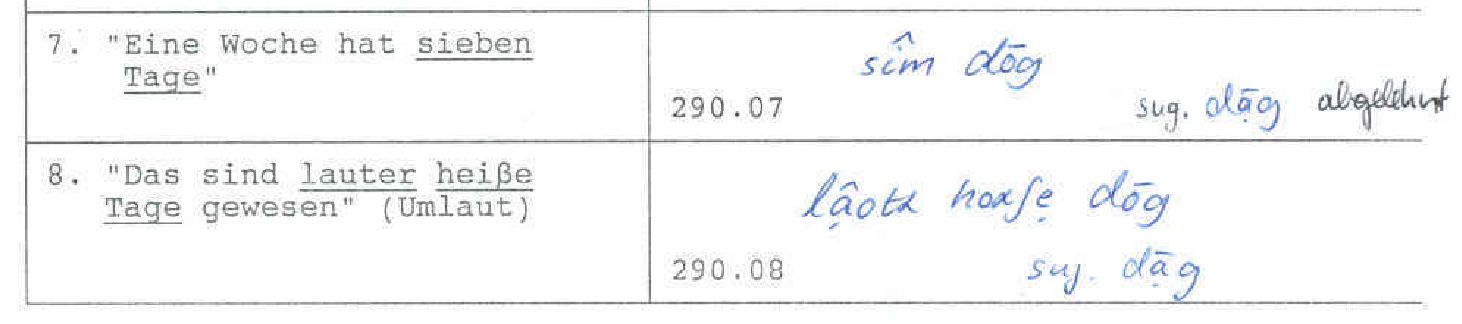
\includegraphics[width=\textwidth]{figures/Fragekontext.png}
\caption{Fragekontext \textit{Tage} im BSA-Fragebuch (nordbair.-mittelbair. Zwiesel)}
\label{fig:17}
\end{figure}

Während diese wenigen Fälle von formaler Variation bei \textit{Baum} und \textit{Bank} Zufallsfunde waren, ermöglichen die BSA-Materialien eine systematische Analyse variierender Pluralformen des Maskulinums \textit{Tag}. Auch hier liegt Variation zwischen Null- und distinkter Markierung vor, etwa in Bernried im nordbair.-mittelbair. Übergangsgebiet: \teuthoo{A}{α} \teuthoo{so4<}{sộ} \teuthoo{A}{α} \teuthoo{s\#e"+nA}{šẽ̄nα} \teuthoo{do<g}{dôɡ} ‚ein so ein schöner Tag‘ -- Pl. \teuthoo{da42g}{dạ̄ɡ} vs. \teuthoo{si."4m}{sị̄ͅm} \teuthoo{do9.<g}{do\klammeruntenpost{}̂ͅɡ} ‚sieben Tage‘. Bemerkenswert sind dabei die Antworten der Gewährsperson aus Zwiesel, ebenfalls nordbair.-mittelbair. Übergangsgebiet. Im Fragekontext ‚lauter heiße Tage‘ hat sie Nullplural produziert und die suggerierte Form mit Umlaut akzeptiert, im Kontext ‚sieben Tage‘ hat sie ebenfalls Nullplural produziert, die suggerierte Umlautform \teuthoo{da24g}{dạ̄ɡ} aber abgelehnt (\figref{fig:17}). Eine Auswertung dieser beiden Fragekontexte in allen SNiB-Erhebungsorten (n= 209) ergibt zwar in diesem Teil des Mittelbair. keine Raumbildung des Phänomens, zeigt aber zwei Haupttypen auf: (1) in beiden Fragekontexten eine „konstante“ Pluralform (Null oder Umlaut oder beide Verfahren als Varianten, 57\,\%).\footnote{Im Einzelnen setzt sich dieser „konstante“ Typus folgendermaßen zusammen: Mehrheitlich ($n=101$, 48\,\%) erscheint Nullplural in beiden Abfragekontexten, sieben Umlautplurale in beiden Kontexten (3\,\% aller Fälle), in zwölf Fällen wurde in beiden Abfragekontexten Null- und Umlautplural realisiert (6\,\%).} (2) Die Gewährsperson produziert oder akzeptiert den Umlautplural nur für die NP ‚lauter heiße Tage‘, in ‚sieben Tage‘ erfolgt Nullmarkierung (40\,\%). (In nur vier Fällen wird Umlautplural im Kontext ‚sieben Tage‘ und Nullplural bei ‚lauter heiße Tage‘ realisiert, <2\,\%.)

Die Verteilung der Varianten des Typs (2) legt hier den Schluss nahe, dass nach Numeralia Nullplural, im Syntagma ‚lauter heiße Tage‘ aber eine dis"-tink"-te Pluralform mit Umlaut realisiert wird. Allerdings hat auch das Adjektivattribut \textit{lauter} eine pluralische Semantik, weshalb sich hier erneut die Frage stellt: Welche semantisch-pragmatischen Kontexte triggern eine dis"-tink"-te Pluralform und wann sind sie (aus Sprecher/Hörer-Perspektive) eindeutig? An dieser Stelle sind die Varianten aus dem mittelbair. Wolfersdorf aufschlussreich. Als isolierte Pluralform realisiert die Gewährsperson den Umlautplural \teuthoo{da42g}{dạ̄ɡ}, im Syntagma ‚lauter heiße Tage‘ hingegen erscheint Nullplural: \teuthoo{la4otA}{lạotα} \teuthoo{ho.ASe4}{hoͅαʃẹ} \teuthoo{do.2g}{dōͅɡ} (die NP mit Zahlwort ist nicht transkribiert).

Da in den BSA-Erhebungen nur zwei Kontexte systematisch abgefragt wurden, muss offenbleiben, wo die Grenze für eine eindeutige vs. uneindeutige Interpretation von Pluralität im semantisch-pragmatischen Zusammenhang liegt. Auch in jenen bair. Dialekten, die in der Datenauswertung in beiden Kontexten (nach Zahlwort und im Syntagma ‚lauter heiße Tage‘) Nullplural haben, kann es potenziell eine fakultative Pluralmarkierung geben; die Semantik von \textit{lauter} war womöglich zu eindeutig, um diese auszulösen. Die Zusammenschau der bisherigen Fälle kontextbedingter formaler Markierung zeigt aber, dass eine dis"-tink"-te Pluralmarkierung bei isolierten Formen oder in Nominalphrasen ohne Artikel erscheint, die formale Markierung also vor allem durch fehlenden morphosyntaktischen Kontext lizensiert ist.

Um ähnliche Forschungsfragen an der Schnittstelle zwischen Flexionsmorphologie und semantisch-pragmatischem Kontext zu beantworten, braucht es weitere Dialektdaten, die (1) die Kontextbedingungen fakultativer Markierungen ausloten, (2) die Möglichkeiten von Face-to-Face-Kommunikation stärker berücksichtigen, als es in einer Interviewsituation möglich ist, und (3) inventarisieren, für welche Substantive eine fakultative Markierung überhaupt zur Verfügung steht. Der historische \textit{a}{}-Stamm \textit{Tag} und der \textit{i}{}-Stamm \textit{Baum} weisen beide lautgesetzlichen Nullplural auf (bei \textit{Baum} durch Zusammenfall der Diphthongreihe mhd. \textit{ei}{}-\textit{öu}{}-\textit{ou} zu \teuthoo{a.}{aͅ}), sie sind diachron in andere (stammaffizierende) Verfahren gewechselt. Sind Deklinationsklassenwechsel hier eine Vorbedingung für die Möglichkeit fakultativer Markierung? Im Falle stammaffizierender Markierung ist dies mit Blick auf die (dürftige) Datenlage nicht auszuschließen. Anders liegt der Fall bei additiven Markierungen, vor allem bei dem im Bair. produktiven Tiefschwa-Suffix (Typ \teuthoo{ba2m}{bām} -- \teuthoo{ba2mA}{bāmα}). Bei \citet[138]{Rowley1997} und \citet[123]{Steininger1994} finden sich Belege für eine fakultative Markierung von \textit{Bube} (\textit{bouma} neben \textit{boum}), \citet[149]{Wildfeuer2001} nennt die Maskulina Akk.Pl. \textit{šręŋαn} ‚Schragen‘ und Akk.Pl. \textit{okßnα} ‚Ochsen‘, die trotz dis"-tink"-ter Artikelformen eine potenzierte Pluralmarkierung aufweisen. Er interpretiert dies als „inter- und intraparadigmatische[n] Ausgleich“, der „zukünftig mehr Wörter erfassen und schließlich regelhaft werden“ könnte (\citealt[149]{Wildfeuer2001}, vgl. \citealt[72]{Mauser2007}).

In dialektologisch-grammatischen Darstellungen wird die fakultative Markierung als besonders frequent bei Feminina mit \textit{n}-Erweiterung im Nom.Sg. angeführt (Typ \teuthoo{das\#n}{dašn} -- \teuthoo{das\#n}{dašn} ‚Tasche‘), da hier auch der Artikel im Nom./Akk. (\textit{die} -- \textit{die}) keine Dis\-am\-bi\-gu\-ie\-rung der synkretischen Numerusformen leistet. \citet[174]{Rowley1997} verortet den arealen „Kern“ der fakultativen Suffigierung von Feminina außerhalb seines nordostbayerischen UGs im Mittelbair. \mapref{map:33} bestätigt dies und zeigt, dass das Gebiet fakultativer Markierung weite Teile des Mittelbair. umfasst und -- so ist zu vermuten -- bis ins östliche Mittelbair. in Österreich hineinreicht (siehe auch \citealt{Mauser2007}).

\begin{map}
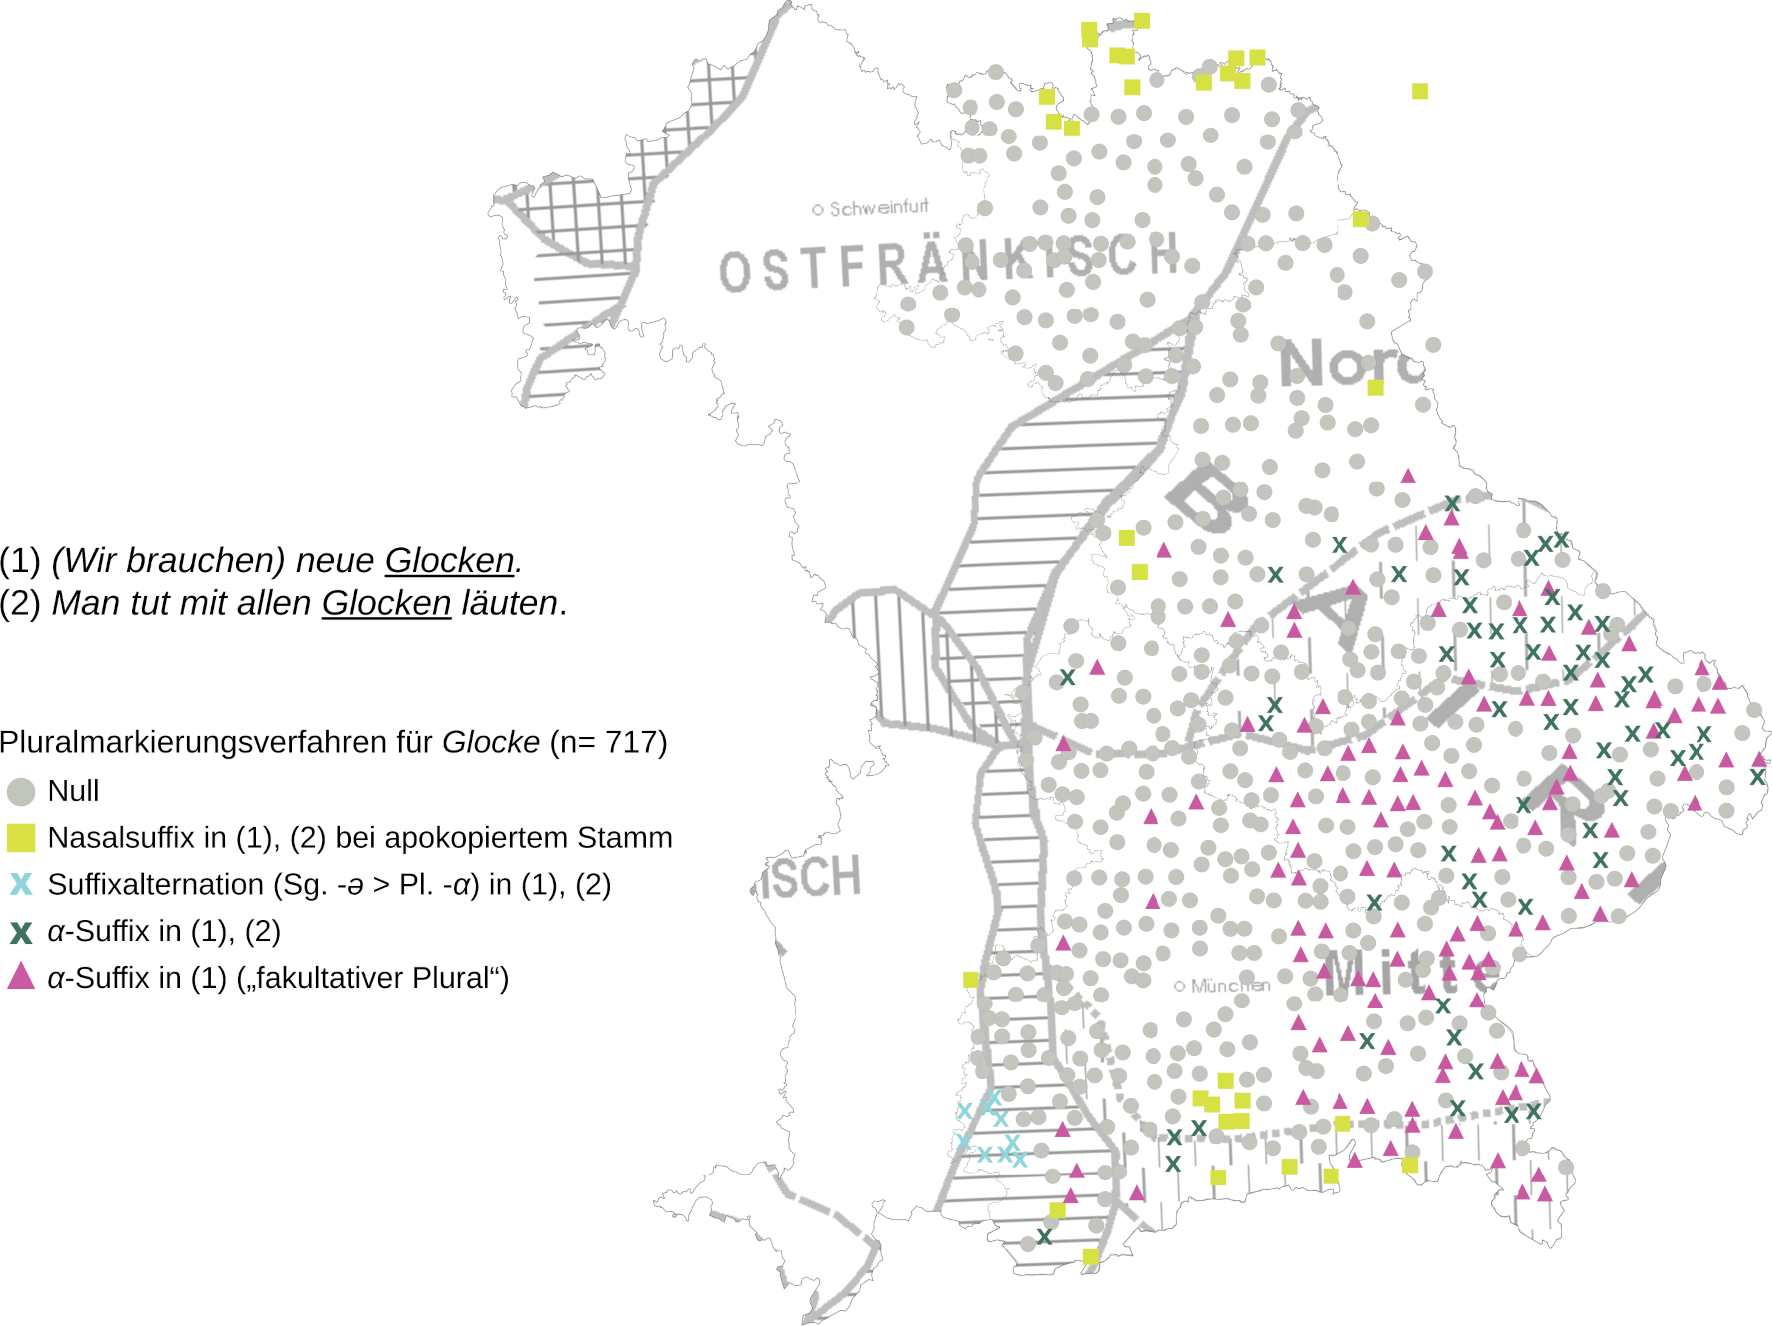
\includegraphics[width=\textwidth]{figures/Karte33.png}
\caption{Fakultative („potenzierte“) Pluralmarkierung bei ‚Glocke‘ in den Daten des SNOB, SNiB und SOB}
\label{map:33}
\end{map}

Kartiert wurden zwei Fragekontexte aus den bair. Teilprojekten SNOB, SNiB und SOB: (1) ‚Wir brauchen neue Glocken‘ und (2) -- mit unbestimmtem Zahlwort -- ‚Man tut mit allen Glocken läuten‘. Das Kartenbild zeigt, dass Nullmarkierung in beiden Kontexten im gesamten UG, d.\,h. im Ofr. und im Bair., belegt und im interdialektalen Vergleich damit ausgesprochen frequent ist. Am nördlichen und südlichen Rand sind nu"-me"-rus"-dis"-tink"-te Formen mit apokopiertem Singularstamm zu finden (Typ \teuthoo{glok}{ɡlok} -- \teuthoo{glokN}{ɡlokŋ}). Ein Spezifikum des mittelbair.-schwäb. Übergangsgebiets im Westen des UGs ist daneben die nu"-me"-rus"-dis"-tink"-te Form mit Suffixalternation: Typ \teuthoo{glokE}{ɡlokə} -- \teuthoo{glokA}{ɡlokα} (siehe \sectref{sec:7.1.1.4}). Im östlichen Mittelbair. und im südlichen Nordbair. finden sich Belege für additive Pluralformen in beiden Fragekontexten (Typ \teuthoo{glokN}{ɡlokŋ} -- \teuthoo{glokNA}{ɡlokŋα}). Ein weitaus größeres Gebiet des Mittelbair. umfassen dagegen die fakultativen Plurale: Eine additive Pluralform findet sich nur in (1), in der NP mit unbestimmtem Zahlwort in (2) ist Nullplural realisiert, z.\,B. \teuthoo{na4ee4}{nạeẹ} \teuthoo{glo4gðnA}{ɡlọɡ̩nα} vs. \teuthoo{mid}{mid} \teuthoo{a.le4}{aͅlẹ} \teuthoo{glo4gðn@}{ɡlọɡ̩n̥} \teuthoo{le.2dn@}{lēͅdn̥} im nordbair.-mittelbair. Blaibach.

In beiden Abfragekontexten erscheint \textit{Glocke} nicht in der Subjektposition, was auch den prototypischen Fall von fakultativen Pluralmarkierungen darstellt. \citet[124]{Steininger1994} findet in seinem Korpus potenzierte Pluralformen vor allem im Akkusativ, im Nominativ gelten sie dagegen „nur mit Einschränkung, da die in der finiten Verbform geforderte Kongruenz ebenfalls die grammatische Kategorie Numerus zum Ausdruck bringt“ (vgl. \citealt[§140.7]{Kollmer1987}, \citealt[159]{Rowley1997}). In den BSA-Daten findet sich indes ein weiterer Beleg fakultativer Markierung, der diese Beobachtung herausfordert. In Bernhardswald (nordbair.-mittelbair. Übergangsgebiet) markiert die Gewährsperson den isolierten Plural von \textit{Sohle} mit Tiefschwa-Suffix (\teuthoo{so24îln}{sọ̄{\aufstrih}ln} -- \teuthoo{so24îlnA}{sọ̄{\aufstrih}lnα}) und bietet für den Satz ‚Beide Sohlen sind hin‘ zwei Varianten: \teuthoo{dso24îlnA}{dsọ̄{\aufstrih}lnα} \teuthoo{sa4n}{sạn} \teuthoo{hi“4}{hị̄} ‚die Sohlen sind hin‘ und \teuthoo{dso24îln}{dsọ̄{\aufstrih}ln} \teuthoo{sa4n}{sạn} \teuthoo{a.îl}{aͅ{\aufstrih}l} \teuthoo{dswôo.u}{dsw{\aufstrih}oͅu} \teuthoo{hi“4}{hị̄} ‚die Sohlen sind alle zwei hin‘. In beiden Fällen dis"-am"-bi"-gu"-iert die Kongruenz zum Verb die Numerusinformation, doch nur in Kombination mit dem Zahlwort entfällt die dis"-tink"-te Markierung am Substantiv. Da es sich um einen einzelnen Beleg\footnote{Das
    Syntagma ‚Beide Sohlen sind hin‘ ist zwar in mehreren BSA-Projekten abgefragt worden, aber bedauerlicherweise liegen die Daten nicht vollständig (bzw. mit fehlerhafter Zuordnung) in der \textit{BayDat} vor, weshalb eine systematische Auswertung ohne Hinzuziehung aller Fragebücher (und idealiter auch der Tonbandaufnahmen) an dieser Stelle möglich ist.}
handelt, ist es nicht unproblematisch, hier grundsätzlich auf die funktionale Bedeutung der Verbkongruenz zur Dis"-am"-bi"-gu"-ie"-rung von Pluralität zu schließen, zumal eventuell auch Intervieweffekte eine Rolle spielen. Der Beleg eröffnet aber in jedem Fall die Frage, ob die Kongruenz zwischen Subjekt-NP und Verb aus Sprecherperspektive ausreichend dis"-am"-bi"-gu"-ie"-rend wirkt oder ob die Pluralität präferiert im nominalen Bereich angezeigt wird. Um Fragen wie diese zu überprüfen, braucht es Erhebungsdaten, die fakultative Markierungen evozieren und neben semantisch-pragmatischen auch noch stärker syntaktische Bedingungen in den Blick nehmen.
